\documentclass[a4paper]{article}
%\usepackage{simplemargins}

%\usepackage[square]{natbib}
\usepackage{amsmath}
\usepackage{amsfonts}
\usepackage{amssymb}
\usepackage{graphicx}
\usepackage{times}
\usepackage{siunitx}
\usepackage{float}
\usepackage[
  sorting=none,
  natbib=true,
  style=numeric-comp,
  maxnames=99
]{biblatex}
\usepackage{xcolor}
\usepackage{hyperref}
\hypersetup{hidelinks,
    colorlinks=true,       
    linkcolor= red!70!black,
    citecolor= red!70!black,        
    filecolor= red!70!black,      
    urlcolor = red!70!black}

\addbibresource{refs.bib}
\AtBeginBibliography{\small}

\DeclareFieldFormat[article]{title}{#1}

\DeclareBibliographyDriver{article}{%
  \printnames{author}. %
  \newblock%
  \printfield{title}. %
  \newblock%
  \href{\thefield{url}}{%
   \itshape%
    %\usebibmacro{journal+issue}%
    \usebibmacro{journal}%
    \setunit*{\addspace}%
    {\bfseries\printfield{volume}}%
    \setunit*{\addcomma\space}%
    %\usebibmacro{issue+date}
    %\setunit{\space}%
    \printfield[noformat]{pages}%
    %\printlist{publisher}% NK wanted removed for academic CV
    \setunit*{}
     (\printfield{year})%
  }
}


\begin{document}
\pagenumbering{gobble}

\Large
 \begin{center}
\textbf{Light scattering from a quantum-degenerate Bose gas}\\

\hspace{10pt}

% Author names and affiliations
\large
Matthew Chilcott$^1$,  Susi Otto, Amita Deb, Niels Kj{\ae}rgaard \\

\hspace{10pt}

\small
Dodd-Walls Centre,  
Department of Physics, University of Otago\\
$^1$ matthew.chilcott@otago.ac.nz\\
\end{center}

\hspace{1pt}
\normalsize
In recent experiments demonstrating Pauli blocking of light scattering from quantum degenerate Fermi gases, we made use of similarly prepared bosons as a benchmark \cite{Deb2021}. In contrast to the monotonic decrease of light scattering encountered for fermions entering the degenerate regime, bosons below the critical temperature $T_C$ for Bose-Einstein condensation display a peaked increase of light scattering \cite{Morice1995,Bons2016}. The enhancement which is tied to an increase in the imaginary part of the refractive index for a Bose gas around $T_C$, was observed in connection to the study \cite{Deb2021}, both as a reduction in transmitted probe light and as an increase in fluorescence as measured on an EMCCD camera. Here we extend our bosonic fluorescence measurements into the time domain, using a single photon counting module. We present recent results that provide a unique window into the dynamics of light scattering from a degenerate gas as it gradually heats up and become thermal.



%Understanding atom-light interactions has been critical to the
%development of modern quantum mechanics, and it remains an active area
%of research. The way ultracold indistinguishable particles scatter
%light has been theorised for a long time, though only recently have
%corresponding measurements made it to the literature, especially the
%suppression of scattering in a near-degenerate gas of Fermions. We
%instead report observations of the corresponding enhancement in light
%scattering off Bosons. This allows us to witness the ``boiling'' of a
%Bose-Einstein condensate (BEC).

\vfill

\begin{center}
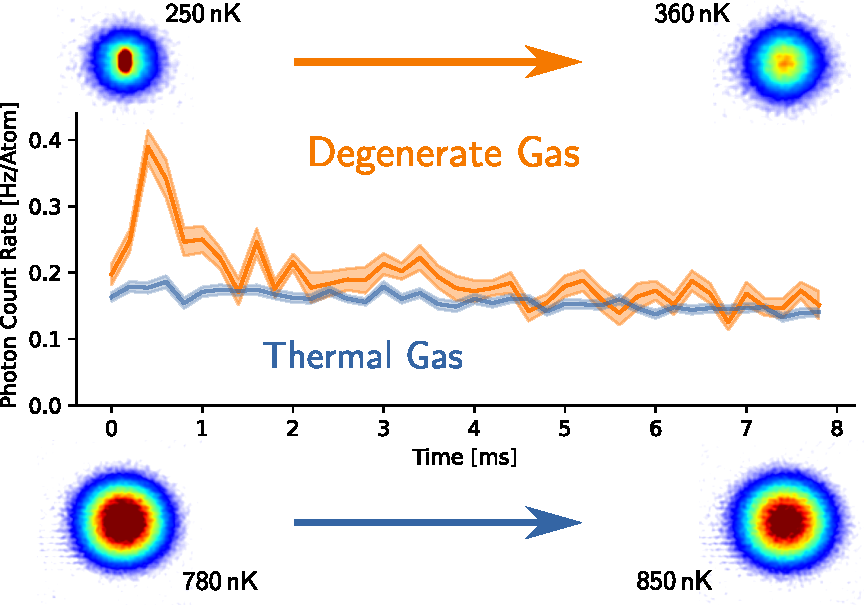
\includegraphics[width=\linewidth]{Figure.pdf}
\end{center}

\vfill

\printbibliography[heading=none]


\end{document}
